\documentclass[11pt,a4paper]{article}

\usepackage[margin=2.4cm]{geometry}
\usepackage[T1]{fontenc}
\usepackage[utf8]{inputenc}
\usepackage{lmodern}
\usepackage{microtype}
\usepackage{graphicx}
\usepackage{booktabs}
\usepackage{tabularx}
\usepackage{array}
\usepackage{amsmath}
\usepackage{xcolor}
\usepackage[numbers,sort&compress]{natbib}
\usepackage[hidelinks]{hyperref}
\usepackage{caption}
\captionsetup{font=small,labelfont=bf}
\setlength{\parindent}{1.2em}
\setlength{\parskip}{0.25em}
\renewcommand{\arraystretch}{1.12}

\title{\bfseries Beyond Candidate Generation: A Validation-First Protocol for AI-Assisted Transition-State Discovery}

\author{
Hao-Fan Li\\[3pt]
\small State Key Laboratory of Structural Chemistry,\\
\small Fujian Institute of Research on the Structure of Matter,\\
\small Chinese Academy of Sciences, Fuzhou 350002, China\\
\small University of Chinese Academy of Sciences, Beijing 100049, China
}
\date{October 2026}

\begin{document}

\maketitle

\begin{abstract}
\sloppy
Machine-learned models can now propose three-dimensional transition-state (TS) geometries in seconds, but a candidate geometry is not a validated TS. The gap between a plausible structure and a mechanistically meaningful barrier---one imaginary frequency, the intended atom pair, the correct connectivity, and a consistent electronic state---remains the bottleneck in AI-assisted computational chemistry. We present a validation-first protocol that separates candidate generation from physical validation. The protocol combines (i) a chemical preflight that fixes reactive pairs, spin surfaces, connectivity, and conformers; (ii) a per-point independent scan that localizes the barrier without fragile collective scans; (iii) a constrained reference calculation that produces the Hessian used for OptTS; and (iv) a validation stage based on imaginary-mode localization, key bond lengths, IRC endpoints, spin diagnostics, and energy-convention checks---preceded by an optional learned-potential pre-screen that repairs malformed candidates and, inside its applicability domain, rejects basin-like guesses before any DFT is spent. The protocol is implemented as a portable, open-source skill package for local ORCA/xtb and Gaussian/Slurm execution. Case studies from Ni/Fe catalysis illustrate where AI helps---multi-sample candidate generation, conformer enumeration, and orchestration---and where it fails: an 84-atom broken-symmetry organometallic system produced candidates with 3.6--4.4~\AA{} heavy-atom RMSD, while a per-point scan strategy completed 16/16 points after a collective scan failed three times. We argue that the near-term role of AI is not to replace electronic-structure judgment but to shrink the search space before it and to make the validation layer reproducible.
\end{abstract}

{\raggedright \noindent\textbf{Keywords:} transition-state discovery; AI-assisted chemistry; automated workflows; DFT validation; reaction mechanisms; reproducibility\par}

\section{Introduction}

Artificial intelligence has changed the practice of computational chemistry. Deep networks plan synthetic routes \citep{Segler2018}, machine-learned potentials reproduce quantum-chemical energy surfaces at a fraction of the cost \citep{Behler2007,Unke2021}, and structure-prediction models have shown how far a learned prior can carry a difficult geometric problem \citep{Jumper2021}. In each case, the model does not replace the underlying physics. It proposes a structure, a route, or a trajectory, and a downstream physical or experimental check decides whether the proposal is meaningful.

Transition-state (TS) discovery is now entering the same pattern. A recent generative model, UniTS-Gen, takes a two-dimensional molecular graph and a set of reactive-atom indices and produces three-dimensional TS guesses \citep{Xu2026UniTS}. The reported accuracy is encouraging but not absolute: most single samples converge to a first-order saddle, and a substantial fraction survive human filtering and IRC validation. The natural response is to generate more samples. The less discussed question is what to do with them. A generated geometry can look like a TS, optimize without error, and still describe the wrong reaction. The missing layer is not a better generator; it is a validation protocol that is model-agnostic, staged by cost, and explicit about failure.

The stakes are high because a TS is not a point cloud. It is a statement about the electronic surface and about connectivity. In homogeneous catalysis, a barrier enters the energy span of a cycle \citep{Kozuch2011Span}, the degree of rate control \citep{Campbell2017DRC}, and the branching ratio between competing channels. A false TS can reverse the ordering of two mechanisms, change a predicted selectivity, or hide a lower-energy pathway. The error is not cosmetic; it propagates into the mechanistic claim.

Current AI-for-TS papers understandably emphasize generation accuracy, because that is what the model contributes. Validation is often described as a system-specific pipeline: a constrained optimization here, a frequency calculation there, an IRC if time permits. That pipeline is difficult to reproduce, difficult to transfer to another laboratory, and easy to skip when a job converges. The result is a gap between what the model can propose and what the community can trust.

This paper argues for a validation-first protocol. The protocol has four mandatory stages---a chemical preflight, a barrier-region scan, a constrained reference calculation that produces the Hessian, and a validation stage---plus an optional learned-potential pre-screen before the scan. Each stage has a gate; each gate has a specific exit; failure at a gate is treated as data rather than as a reason to restart. The protocol is implemented as a portable, open-source skill package that runs local ORCA/xtb and Gaussian/Slurm jobs, and it is illustrated with internal case studies from Ni/Fe catalysis. The contribution is not a new model. It is the layer that makes a model's output scientifically usable.

The scope is deliberately narrow. The protocol targets a defined elementary step in a single-reference DFT setting, typically 50--120 atoms, with an organic or organometallic system. It does not cover excited-state or nonadiabatic dynamics, strong multireference systems, or transport-limited reactors. Those are important problems, but they require different validation criteria. The claim is also modest: the protocol reduces false positives and makes the remaining uncertainty visible. It does not eliminate method error, and it does not discover the mechanism for the user.

\section{What makes a transition state a transition state}

A first-order saddle on a potential-energy surface has three properties. It has exactly one imaginary vibrational frequency; the corresponding normal mode points along the reaction coordinate; and the two steepest-descent paths from the saddle connect the intended reactant and product. A candidate geometry has none of these properties by construction. It is a hypothesis about where the saddle might be.

The distinction matters because a single imaginary frequency is a necessary but not sufficient condition. A point can have one imaginary frequency and still be the wrong channel: the mode may involve a spectator ligand, a proton transfer that was not intended, or a different bond altogether. It can also be a second-order saddle with two imaginary frequencies, one of which is a soft spectator mode that is easy to dismiss as numerical noise. It can be a flat transition valley with several shallow imaginary modes, in which case a single saddle may not exist on the chosen surface. Each of these outcomes can survive a visual inspection and a successful optimization.

A barrier is also meaningless without a reference state. The same TS geometry can be assigned different barriers depending on the reactant, the encounter complex, the electronic state, and the energy convention. For a catalytic cycle, the relevant quantity is not an isolated barrier but the energy span between the highest transition state and the lowest intermediate that precedes it \citep{Kozuch2011Span}; the degree of rate control then identifies which step actually controls the rate \citep{Campbell2017DRC}. A wrong TS changes the span and can change which step is controlling. At the level of competing channels, the product ratio is a flux branching ratio, not a Boltzmann ratio over product free energies, unless the products equilibrate on the observation timescale. The validation protocol therefore has to check not only the saddle but also the reference state and the connectivity.

The physical picture behind these checks is standard. Transition-state theory relates the rate to the barrier \citep{Eyring1935}; the barrier itself varies with the driving force \citep{EvansPolanyi1938}; Kramers theory adds friction and recrossing \citep{Kramers1940}; Marcus theory makes the driving-force dependence explicit for electron transfer \citep{Marcus1956,Marcus1993}. Nonequilibrium thermodynamics adds the constraint that a net flux cannot run against the affinity \citep{Onsager1931}, and fluctuation theorems make the free-energy difference a functional of the work distribution \citep{Jarzynski1997,Crooks1999,Seifert2012}. For a reaction network, the topology can enforce a unique steady state independent of the rate constants \citep{Feinberg1987}. These results do not remove the need for a validated TS; they explain why the validation must include the reference state, the direction of the flux, and the connectivity.

The practical consequence is that validation is a classification problem with expensive labels. A candidate can fail at the level of the electronic structure (wrong spin state, wrong oxidation state, wrong method), at the level of the geometry (wrong channel, wrong conformer, second-order saddle), or at the level of the energy accounting (wrong reference, mixed solvation convention, $\Delta E$ versus $\Delta G$). The protocol in the next section orders these checks by cost, so that most candidates fail before the most expensive calculation.

\section{A validation-first protocol}

The protocol is summarized in Figure~\ref{fig:workflow}. It separates the generator from the validator. The generator can be a machine-learned model, an automated search, or a human guess; the validation layer is unchanged. The four mandatory stages are described below, together with one optional accelerator (P0.5), and the stop rules are collected in Table~\ref{tab:stop}.

\begin{figure}[t]
\centering
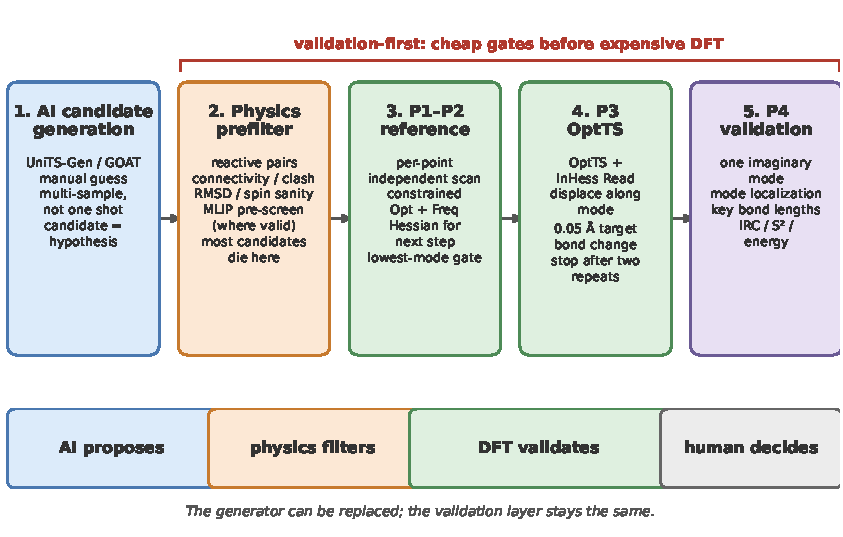
\includegraphics[width=0.98\linewidth]{figures/workflow.pdf}
\caption{A validation-first protocol for AI-assisted TS discovery. Candidate generation (left) is separated from physical validation (right). The cheap gates, including an optional learned-potential pre-screen, reject most candidates before the expensive OptTS step. The generator can be replaced without changing the validation layer.}
\label{fig:workflow}
\end{figure}

\paragraph{P0: chemical preflight.}
Before any quantum-chemical job, five declarations are written down. First, the reactive pairs: which bonds form and which break, with their actual distances in the starting geometry. A pair at 4.5~\AA{} is usually a mistake. Second, the charge, multiplicity, and spin surface. For a transition metal, every accessible $d^n$ state is listed, including broken-symmetry solutions; a TS is then sought on each surface rather than on a default. Third, connectivity: a bond graph is built with a distance criterion, and the intended bonds are checked against the graph, together with any unplanned bond. Three real projects were lost to a ``reactant'' that had already rearranged. Fourth, conformers: flexible ligands and chains are pre-folded with a cheap method, and several low-energy conformers are retained. A single-conformer R/S difference can be dominated by the conformer, not by the stereochemistry. Fifth, the reference state: the reactant or encounter complex and the product, at the same level as the TS. A barrier without a defined reference is not a barrier.

The preflight also includes a candidate filter: hard overlaps, clash ratios, heavy-atom RMSD to a reference, and connectivity changes. The filter is deliberately conservative. Its purpose is not to decide which candidate is correct; it is to make the expensive stage affordable. In the implementation, the filter is a separate script so that it can be used with any generator.

\paragraph{P0.5: learned-potential pre-screen (optional).}
Before the barrier scan, the candidate can be passed through a foundation machine-learned potential \citep{Husistein2026Paradigm,Neumann2024Orb,Levine2025OMol25}. The screen is deliberately restricted to geometry: the candidate is displaced along the declared reaction coordinate in both directions and relaxed on the learned surface. If both descents reach the same minimum, the candidate is basin-like and is discarded; if they differ by exactly the declared forming and breaking bonds, it is barrier-like and passes to P1; if they differ in any other way, the reactive pairs are re-examined. The same tool repairs malformed starts: hard overlaps of 0.83--0.93~\AA{} are removed and the declared bonds are pulled to their target lengths while the coordination sphere is held. The stage is optional because its validity is system-dependent. On our broken-symmetry organometallic systems it does not support the reaction at all: all five DFT-validated saddles were flagged as lying 83--85 kcal mol$^{-1}$ above both endpoints, with both descents collapsing to the coupled product, whereas a DFT minimum was correctly classified as basin-like. We therefore use it as a geometry-repair tool on those systems, and as a candidate gate only where the electronic state lies inside the model's applicability domain. It does not save DFT cycles by satisfying constraints: ORCA projects the constraints onto the input geometry before the first optimization cycle (measured, Ni--C$^*$ 3.000 $\rightarrow$ 2.150~\AA{}), and the hundreds of cycles that follow are ligand-conformer relaxation, which the screen does not replace.

\paragraph{P1: barrier-region scan.}
A blind OptTS is the most expensive way to test a guess. The protocol instead scans the reaction coordinate with a small number of points. In ORCA \citep{Neese2012ORCA}, each point is an independent \texttt{!Opt} job with the reactive distance constrained, starting from the previous converged geometry. This design is not cosmetic. In our tests with ORCA 6.1.1, a collective relaxed scan failed whenever any single point hit \texttt{MaxIter}: the archive step failed repeatedly and the remaining points never ran. Running each point as its own job makes a failed point local. A 16-point profile that had repeatedly destroyed collective scans completed 16/16 points with this strategy, including the point that had failed twice before.

Only converged points enter the profile. The highest converged point is used as the guess for the next stage; the shape of the profile is used to decide whether the channel is monotonic, whether there is a shallow double bump that signals a conformer change, or whether the channel is a flat valley. The scan is not a TS search. It buys a good guess and a barrier shape at a cost that is small compared with a failed OptTS.

For Gaussian \citep{Gaussian16}, the same idea is implemented with a sequence of \texttt{opt=modredundant} constrained optimizations, each reading the previous geometry. The engine changes; the staging does not.

\paragraph{P2: constrained reference and Hessian.}
At the highest point of the profile, a constrained optimization with a frequency calculation is run. This produces two assets. The first is a reference point: a minimum on the constraint surface, not a stationary point of the full surface. It is already useful for relative comparisons if the next stage fails. The second is an analytic Hessian, which is the input to the TS optimization.

The gate is the mode spectrum. The lowest modes at the constrained point must involve the declared reactive pair. If they do not, the point is not on the intended reaction coordinate, and running OptTS would give the optimizer the wrong mode. The correct response is to change the constraint, the conformer, or the guess; increasing \texttt{MaxIter} is not a response. This gate is cheap and catches a large fraction of wrong guesses.

\paragraph{P3: OptTS with Hessian reuse.}
The TS optimization reads the Hessian from P2. In ORCA this is \texttt{InHess Read} with the Hessian file; in Gaussian it is \texttt{opt=(ts,readfc,noeigen)} with a checkpoint from the constrained calculation. Without this step, ORCA falls back to a model Hessian and can climb the wrong mode for hundreds of cycles. The Hessian is the most reusable asset in the workflow, and reusing it is the single largest reliability gain.

If a displacement is needed, it is made along the imaginary mode, but the amplitude is scaled by the target bond-length change, not by the maximum atomic displacement. A displacement of 0.18~\AA{} in the maximum atomic coordinate can change the reactive bond by $-0.31$~\AA{} and throw the geometry into the reactant basin; a target bond change of about 0.05~\AA{} keeps the geometry in the saddle neighborhood. The distinction is quantitative and easy to miss.

The optimization is also governed by stop rules. If the energy decreases monotonically for more than about 50 cycles and the reactive bond is unchanged, the start is in the wrong basin. If two displaced optimizations return to the same geometry and energy, the point is a second-order saddle or a flat valley, and a third attempt is unlikely to help. These rules are listed in Table~\ref{tab:stop}.

\paragraph{P4: validation.}
The final stage asks whether the candidate is a TS for the intended reaction. The checks are ordered by informativeness. First, the number of significant imaginary frequencies: exactly one for a first-order saddle. Second, the localization of the imaginary mode: the transferring atom should account for a substantial fraction of the displacement; a delocalized mode below about 15\% is a spectator or soft-mode artifact. Third, the key bond lengths: a saddle with one imaginary frequency and the declared atom pair can still be a different channel. Fourth, connectivity: an IRC in both directions, or a downhill relaxation as a cheaper substitute, must reach the intended reactant and product. Fifth, the spin diagnostics: $\langle S^2\rangle$ and the Mulliken spin density must be consistent with the geometry's electronic state, and a broken-symmetry single point must inherit the full broken-symmetry setup. Sixth, the energy convention: optimization, frequency, and IRC at the same level; $\Delta E$ for a minimum-versus-saddle comparison; one solvation convention across all species.

The validation stage is not designed to prove that the calculation is right. It is designed to make the failure modes visible. A candidate that passes all six checks is not guaranteed to be the true mechanism, but it is a defensible TS at the stated level of theory. A candidate that fails one check is not automatically wrong, but the failure has to be explained rather than ignored.

\begin{table}[t]
\centering
\caption{Stop rules used in the protocol. Each rule routes a failed candidate to a specific action rather than a blind restart.}
\label{tab:stop}
\small
\begin{tabularx}{\linewidth}{@{}p{0.4cm}>{\raggedright\arraybackslash}X >{\raggedright\arraybackslash}X@{}}
\toprule
\# & Symptom & Action \\
\midrule
1 & Lowest mode at P2 does not involve the reactive pair & Do not run OptTS; change the constraint, conformer, or guess \\
2 & OptTS energy decreases monotonically for $>50$ cycles while the reactive bond is unchanged & Wrong basin; stop and return to P1/P2 \\
3 & Two displaced OptTS runs return to the same geometry and energy ($<0.01$ kcal mol$^{-1}$) & Stop; accept with disclosure, rigidify the spectator, or run IRC along the reactive mode \\
4 & Two or three shallow imaginary modes around $-15$ to $-25$ cm$^{-1}$ & Flat transition valley; use the last geometry's frequency as a reference barrier and say so \\
5 & Imaginary-mode localization below 15\% & Delocalized soft mode, not the target coordinate \\
6 & \texttt{SADDLE-1} and the declared pair matches, but key bond lengths are wrong & Wrong channel; do not report this barrier \\
7 & IRC or relaxation endpoint is not the intended reactant/product & No barrier claim; return to P1/P2 \\
8 & Single-point $\langle S^2\rangle$ differs from the geometry job & Wrong electronic state; repeat the full spin setup \\
9 & R/S difference without a conformer search & Not a stereoselectivity result; do the ensemble first \\
10 & xtb and DFT disagree & DFT wins; xtb is for folding only \\
11 & MLIP candidate lies $>60$ kcal mol$^{-1}$ above both relaxation endpoints (PES mismatch) & Do not treat it as a basin; skip the screen and go to P1 \\
\bottomrule
\end{tabularx}
\end{table}

\section{What AI contributes---and what it does not}

\subsection{Candidate generation}

The most mature contribution is candidate generation. UniTS-Gen reports that most single samples converge to a first-order saddle and that about 42\% survive filtering and IRC \citep{Xu2026UniTS}. Those numbers are useful for expectation management, not for deciding whether a particular candidate is correct. The intended use is multi-sampling: generate ten candidates, reject most of them with the physics filter, and send only a few to DFT. In the published benchmark, ten samples per case recovered all five previously failed cases \citep{Xu2026UniTS}. The gain comes from coverage, not from a guarantee.

The failure mode is equally informative. In an internal test on an 84-atom Ni broken-symmetry organometallic system, four generated candidates passed the geometric filter, but their heavy-atom RMSD to the reference was 3.6--4.4~\AA{}, and none had both the Ni--C bond and the incipient C$\cdots$C contact of the intended S$_H$2 step. The model was out of distribution: large, flexible, open-shell, and transition-metal-rich. The practical rule is not ``never use a generative model''; it is ``use it where it has been validated, and prefer a hand-built guess plus the protocol where it has not.''

ORCA's GOAT-TS mode is a useful non-ML alternative. It explores structures and reaction channels with the electronic-structure method itself, so it does not inherit a training-set bias. The cost is CPU time, and it becomes expensive for large flexible systems. It is best used to check whether a channel exists, or to generate a guess for a medium-sized system, not as a production TS optimizer for a 100-atom catalyst.

\subsection{Conformers and surrogate barriers}

Machine-learned potentials and cheap semiempirical methods are useful for conformer enumeration \citep{Behler2007,Unke2021}. They can generate and rank conformers at a cost that is negligible compared with DFT, and they can reveal that a single-conformer R/S difference is dominated by the conformer. Learned coarse-grained dynamics can play a similar role for slow conformational transitions \citep{Mardt2018}. In one internal case, the ligand-overlay RMSD between the R and S intermediates was 1.62~\AA{}, which is larger than the structural difference one would attribute to the stereocenter. The lesson is not that the conformer search decides the selectivity; it is that the conformer search must precede the selectivity claim.

Surrogate barriers are useful for ranking, not for reporting. A machine-learned potential or a $\Delta$-ML correction can tell us which of two channels is likely to be lower, and can prioritize the DFT jobs. It cannot, at present, deliver a 1 kcal mol$^{-1}$ transition-metal barrier with calibrated uncertainty. The protocol therefore uses surrogates only before P2, and never as the final number. We tested this directly \citep{Neumann2024Orb,Levine2025OMol25}. On five DFT-validated S$_H$2 saddles, a foundation potential placed the candidate 83--85 kcal mol$^{-1}$ above both relaxation endpoints and relaxed the biradical straight to the coupled product; on a DFT minimum it correctly returned a basin. The useful roles are therefore (i) repair of malformed starts and (ii) rejection of basin-like guesses, and only inside the model's applicability domain. A learned potential that has never seen the electronic state cannot rank the channels of that state.

\subsection{Orchestration}

A less glamorous but reliable contribution is orchestration. Generating inputs, parsing outputs, checking convergence, and monitoring a queue are repetitive and error-prone. A script or an agent can reduce format errors and prevent the classic failure of running two quantum-chemistry jobs at once. It can also make the workflow reproducible: the same command sequence, the same gates, and the same report. In our experience, this layer saves more wall-clock time than a better generator, because it prevents the 10--20 h dead ends that come from a wrong start or a missed convergence check.

\subsection{The division of labor}

Table~\ref{tab:ai} summarizes the division of labor. AI proposes; physics filters; DFT validates; the human decides. The human is not a ceremonial approver. The human defines the elementary step, enumerates the spin surfaces, judges whether a channel is chemically plausible, and decides how to report a negative result. The protocol is designed to make those decisions explicit, not to automate them away.

\begin{table}[t]
\centering
\caption{What AI and automation contribute to TS discovery, and what they do not.}
\label{tab:ai}
\small
\begin{tabularx}{\linewidth}{@{}p{3.0cm}>{\raggedright\arraybackslash}X >{\raggedright\arraybackslash}X@{}}
\toprule
Role & Contribution & Limit \\
\midrule
Candidate generation & Multi-sample 3D guesses; coverage of conformers and channels & Single-shot accuracy is moderate; large broken-symmetry organometallics are out of distribution \\
Conformer enumeration & Cheap pre-folding and ranking; exposes conformer-dominated differences & Does not decide which conformer controls selectivity \\
Surrogate barriers & Ranking of channels; prioritization of DFT jobs & Not a quantitative transition-metal barrier at 1 kcal mol$^{-1}$ \\
Orchestration & Input generation, parsing, monitoring, reproducibility & Does not validate the electronic structure or the mechanism \\
Learned-potential pre-screen & Removes overlaps; rejects basin-like candidates inside its domain & Broken-symmetry organometallics are outside the domain; no quantitative barrier \\
\bottomrule
\end{tabularx}
\end{table}

\section{Case evidence from Ni/Fe catalysis}

The protocol was developed in the context of Ni/Fe-catalyzed decarboxylative coupling and S$_H$2-type bond formation \citep{Tsymbal2022SH2}. The systems are 84--98 atoms, contain one or two transition metals, and often require broken-symmetry or open-shell solutions. The case studies below are internal observations, not a controlled benchmark. They are reported because they illustrate the failure modes that the protocol is designed to catch.

\paragraph{Per-point scans versus collective scans.}
A 16-point radical-attack profile was attempted with a collective relaxed scan. The scan failed three times. The failure was not caused by memory or disk: one point hit the optimization limit, and the archive/cleanup chain then failed for the whole scan. Replacing the scan with independent constrained optimizations completed all 16 points, including the point that had failed twice; that point converged in 44 cycles. The lesson is that a fragile collective operation should not be the unit of failure. A per-point job makes the failure local and the profile salvageable.

\paragraph{Displacement amplitude.}
In a six-membered-ring S$_H$2 TS, a distorted start was generated by displacing along the imaginary mode with a target maximum atomic displacement of 0.18~\AA{}. The actual reactive bond changed by $-0.31$~\AA{}, and the optimization ran for 183 cycles monotonically into the reactant basin. Rescaling the displacement to a target bond change of about 0.05~\AA{} placed the geometry in the saddle neighborhood. The lesson is that mode displacement should be defined in the coordinate that matters, not in the largest Cartesian component.

\paragraph{Second-order saddle.}
The same six-membered-ring TS retained two imaginary frequencies after the first refinement: a large coupling mode and a smaller spectator mode. Two rounds of displacement along the spectator mode returned to the same geometry and energy, within 0.003 kcal mol$^{-1}$, and a finer integration grid confirmed that the soft mode was real rather than a grid artifact. A third round would have repeated the same trajectory. The protocol's stop rule is to accept the point with disclosure, rigidify the spectator, or run IRC along the reactive mode; it is not to restart the optimizer.

\paragraph{Conformer-dominated R/S differences.}
The R and S intermediates of a chiral Ni complex differed by a ligand-overlay RMSD of 1.62~\AA{}. The two structures were not related by a simple stereochemical inversion; they occupied different pockets. A single-conformer R/S energy difference in such a system is not a stereoselectivity prediction. The protocol requires a conformer search and a population-weighted analysis before any ee claim. This is a case where the most important validation is not the frequency calculation but the conformational ensemble.

\paragraph{Generative model out of distribution.}
The 84-atom Ni broken-symmetry test described above produced four candidates that passed the geometric filter but had 3.6--4.4~\AA{} heavy-atom RMSD to the reference. The candidates were not random noise; they were plausible-looking structures in the wrong pocket. The lesson is that a geometric filter is necessary but not sufficient, and that a generative model's applicability domain has to be tested on the system class, not assumed from a benchmark on smaller organic molecules.

\paragraph{Learned-potential pre-screen: where it helps and where it does not.}
The pre-screen was tested against seven structures whose status had already been fixed by DFT: five S$_H$2 saddles ($-574$ to $-581$ cm$^{-1}$, 84--98 atoms, broken-symmetry singlets) and one constrained minimum. The minimum was classified correctly as basin-like. All five saddles fell outside the learned surface: the MLIP energy at the DFT geometry was 83--85 kcal mol$^{-1}$ above both relaxation endpoints, and both descents reached the C--C coupled product rather than the radical--metal encounter. The model does not represent the broken-symmetry state, so no verdict is possible; we record the outcome as a PES mismatch and pass the candidate to P1. As a geometry repair, the same tool removes 0.83--0.93~\AA{} overlaps in about a minute. The lesson is that a learned potential can shorten the path to a valid start, but it cannot substitute for the electronic-structure judgment that defines the saddle.

\begin{table}[t]
\centering
\caption{Representative case evidence from Ni/Fe catalysis. These are internal case studies, not a controlled benchmark; the numbers illustrate failure modes and are not a claim of general superiority.}
\label{tab:cases}
\small
\begin{tabularx}{\linewidth}{@{}p{3.2cm}>{\raggedright\arraybackslash}X >{\raggedright\arraybackslash}X@{}}
\toprule
Case & Observation & Lesson \\
\midrule
Per-point scan & 16/16 points converged after three collective scans failed; the problematic point converged in 44 cycles & Make the unit of failure local \\
Mode displacement & 0.18~\AA{} maximum displacement changed the reactive bond by $-0.31$~\AA{}; 183 cycles into the reactant basin & Scale by the target bond change ($\sim$0.05~\AA{}) \\
Second-order saddle & Two rounds returned the same geometry and energy (0.003 kcal mol$^{-1}$); a finer grid confirmed the soft mode & Stop after the second repeat; disclose or rigidify \\
Conformer-dominated R/S & Ligand-overlay RMSD 1.62~\AA{} between R and S intermediates & Search conformers before claiming stereoselectivity \\
Generative model OOD & Four candidates passed the filter but had 3.6--4.4~\AA{} RMSD to the reference & Test the applicability domain on the system class \\
Learned-potential pre-screen & 5/5 DFT-validated saddles flagged as PES mismatch (83--85 kcal mol$^{-1}$); a constrained minimum correctly basin-like & Repair geometries with it; gate candidates only inside its domain \\
\bottomrule
\end{tabularx}
\end{table}

\section{Implementation and reproducibility}

The protocol is implemented as a portable skill package. The core scripts use only the Python standard library, so a new user does not need a deep-learning environment to validate a candidate. The optional learned-potential pre-screen (P0.5) is distributed in the same package but requires PyTorch and an OMol25-trained potential \citep{Levine2025OMol25}; it is not on the critical path, and every gate that decides whether a candidate is a TS runs without it. The package includes a candidate filter, a per-point scan generator and runner, ORCA and Gaussian input generators, ORCA and Gaussian output verifiers, a structure preflight checker, and an environment doctor. The doctor checks the Python version, compiles every script, locates ORCA, Gaussian, xtb, Slurm, and SSH, and runs four generator/parser self-tests. It does not run a quantum-chemistry job.

The package is intentionally boring. Inputs are explicit; there is no hidden state; the generated runners check that upstream files exist before starting a downstream job. Local execution is supported for ORCA and xtb; Gaussian is supported locally and through Slurm templates. The cluster-specific values (partition, cores, memory, scratch, Gaussian root) are parameters, not assumptions. The same protocol can be run on a workstation or on a cluster without changing the validation logic.

The repository also includes printable checklists for P0--P4, a failure catalogue, and command templates. These are not documentation for its own sake; they are the operational form of the protocol. A new user can run the doctor, run a five-minute smoke test, and then apply the same gates to a real system.

\section{Discussion}

The protocol suggests a broader lesson for AI in computational chemistry. The value of a model is not only its accuracy on a benchmark; it is the fraction of its output that survives a well-defined validation layer. A model that is 40\% correct but cheap, diverse, and easy to filter can be more useful than a model that is 60\% correct but produces plausible wrong channels that are expensive to reject. The field needs benchmarks at the level of validated mechanisms, not only at the level of generated geometries. It also needs negative results: a candidate that failed IRC, a spin surface that was not accessible, a conformer that changed the selectivity.

Several developments would make the validation layer stronger. Uncertainty quantification and out-of-distribution detection would tell the user when to trust a generated candidate and when to fall back to a manual guess. Mechanism-level benchmarks with IRC-validated TSs would make the comparison between generators meaningful. More data for transition-metal and broken-symmetry systems would reduce the applicability-domain problem. Active learning could choose the next calculation or experiment to maximize information, and autonomous laboratories could close the loop. None of these replaces the validation gates; they make the gates more informative.

The limitations of the present work are real. The case studies come from one group's systems and are not a controlled benchmark. The underlying DFT method has its own errors, typically several kcal mol$^{-1}$ for barriers and transition-metal energetics; the protocol reduces false positives but does not eliminate method error. Conformational entropy, solvation, counterions, and spin-state ordering remain difficult. The protocol is also silent on excited-state and nonadiabatic processes, where a single electronic surface is not the right object. These limitations define the boundary of the claim: the protocol makes a candidate defensible at a stated level of theory, not uniquely correct.

Finally, the protocol is model-agnostic. It can accept a candidate from UniTS-Gen, GOAT, a machine-learned potential, or a human. That is the point. The generator will change; the validation layer should not. In the near term, the most useful role of AI is to shrink the search space before the expensive calculation, and to make the remaining uncertainty explicit. The human still decides what the result means.

\section{Conclusion}

A generated geometry is a candidate, not a transition state. The difference is not a detail: it is the difference between a plausible picture and a mechanistic claim. The validation-first protocol described here separates candidate generation from physical validation, stages the checks by cost, and turns failure into a specific next action. It is implemented as a portable, open-source package for local ORCA/xtb and Gaussian/Slurm execution, and it is illustrated with case studies from Ni/Fe catalysis. The protocol does not replace electronic-structure judgment, and it does not discover the mechanism. It does something more modest and more useful: it makes the output of an AI model testable.

\section*{Data and code availability}

The protocol is implemented in the \texttt{ts-computation-suite} package, available at \url{https://github.com/lhfjjk/ts-computation-suite}. The manuscript uses no experimental data. The case-study numbers are reported in Table~\ref{tab:cases}; the underlying geometries and outputs are available from the corresponding author on reasonable request.

\section*{Author contributions}

H.-F.L. designed the protocol, wrote the software, performed the calculations, analyzed the data, and wrote the manuscript.

\section*{Conflicts of interest}

The author declares no competing financial interest.

\section*{Acknowledgements}

The author thanks colleagues for discussions and acknowledges computational resources from the FJIRSM computing cluster.

\bibliographystyle{unsrtnat}
\bibliography{references}

\end{document}
